\documentclass[]{trbunofficial_bdit_final}

\usepackage{graphicx}
\setkeys{Gin}{keepaspectratio}

% \usepackage[colorlinks=true,linkcolor=blue,citecolor=blue]{hyperref}
% For TRB version hide links
\usepackage[hidelinks]{hyperref}
\def\UrlBreaks{\do\/\do-}
\usepackage[normalem]{ulem}
\usepackage{longtable_bugfix}
\usepackage{booktabs}
\usepackage{amsmath}
\usepackage{amssymb}

\AuthorHeaders{Dumas et al.}
\title{A Comprehensive Investigation into Ridesourcing Company
Activities in Toronto}

\author{%
  \textbf{Raphael Dumas}\\
  Big Data Innovation Team, City of Toronto Transportation Services\\
  703 Don Mills Rd., North York, Ontario, Canada M3C 3N3\\
  raphael.dumas@toronto.ca\\
  \hfill\break%
  \textbf{Chenchong Charles Zhu}\\
  Big Data Innovation Team, City of Toronto Transportation Services\\
  703 Don Mills Rd., North York, Ontario, Canada M3C 3N3\\
  charles.zhu@toronto.ca\\
  \hfill\break%
  \textbf{Jesse Coleman}\\
  Big Data Innovation Team, City of Toronto Transportation Services\\
  703 Don Mills Rd., North York, Ontario, Canada M3C 3N3\\
  jesse.coleman@toronto.ca\\
  \hfill\break%
  \textbf{Rick Liu}\\
  Department of Civil \& Mineral Engineering, University of Toronto\\
  35 St. George Street, Toronto, Ontario, Canada M5S 1A4\\
  rick.liu@mail.utoronto.ca\\
  \hfill\break%
  \textbf{Natalie Chan Ho Man}\\
  Big Data Innovation Team, City of Toronto Transportation Services\\
  703 Don Mills Rd., North York, Ontario, Canada M3C 3N3\\
  natalie.chan@toronto.ca\\
  \hfill\break%
  \textbf{Aakash Harpalani}\\
  Big Data Innovation Team, City of Toronto Transportation Services\\
  703 Don Mills Rd., North York, Ontario, Canada M3C 3N3\\
  aakash.harpalani@toronto.ca
}

\begin{document}
\maketitle

\hypertarget{abstract}{%
\section{Abstract}\label{abstract}}

We present a comprehensive study of how the introduction of ridesourcing
companies such as Uber and Lyft has changed travel patterns and behaviours in
the City of Toronto. Origin-destination data for nearly 100 million trips
between 2016 and 2019 were analyzed to determine spatial and temporal trends
for ridesourcing activity. These data were combined with car travel time,
public transportation network and city bylaw data to investigate the impact
of ridesourcing on the transportation network, public transit and cyclists.
To determine the fraction of total City vehicle kilometres travelled (VKT) due to
ridesourcing vehicles, we routed individual trips, and linked trip drop-off
points with nearby pick-up points to simulate driver deadheading between trips.
We find a three-fold growth in the total number of trips per day, with the
greatest absolute growth situated in downtown Toronto during Friday and
Saturday evenings. The greatest fractional growth, on the other hand, is in
weekday commuter trips in the suburbs. A conservative estimate of ridesourcing
vehicle volumes show they account for \(\sim 5 - 8\%\) of overall daily VKT in
September 2018, roughly a factor of two increase from October 2016. Over a
similar period we find only marginal changes in travel time on downtown Toronto
streets. We analyze curbside pick-up and drop-off data to demonstrate a need to
study further how to improve curbside operations to improve safety.

\hfill\break\%
\noindent\textit{Keywords}: ridesourcing, Uber, Lyft, big data, regulation,
shared mobility, policy analysis

\hypertarget{introduction}{%
\section{Introduction}\label{introduction}}

The growth of ridesourcing companies (alternatively ride-hailing companies or
transportation network companies (TNCs)) such as Uber and Lyft across North
American cities over the past decade has led to enormous and rapid changes in
travel behavior. In March of 2019, an average of 770,000 ridesourcing trips
were performed daily in New York City \cite{schneider2019dashboard} and
330,000 in Chicago \cite{chicago2019transportation}. Despite its prevalence,
how ridesourcing contributes to congestion, impacts other road users, interacts
with public transportation and affects transportation equity all remain topics
of active debate amongst researchers, city planners and policy-makers. This is
in part because details and data records of ridesourcing company operations are
generally kept private, forcing researchers to use novel means of collecting
them, such as scraping vehicle position data using APIs provided by the
companies (\trbcite{cooper2018profiling}) or even driving for the companies
themselves (\trbcite{henao2018impact}). Consequently, cases where companies
volunteer disaggregated trip data or submit it for regulation (eg.
\trbcite{rideaustin2017data}; companies in New York City \cite{nyctlc2019report})
make for unique opportunities to build comprehensive pictures of how they
operate within a city.

Uber first started offering its UberX service in Toronto, Canada, in September
2014. In response to growth in ridesourcing activity, in July 2016, the City of
Toronto amended the Vehicle-for-Hire (VFH) Bylaw \cite{vfhbylaw} that regulates
taxis and limousines to enable ridesourcing services to operate in the city by
September 2016. This bylaw requires ridesourcing companies to report individual
trip origin-destination (OD) data to the city. Lyft followed Uber into the
Toronto market at the end of 2017.

In 2018, the City undertook a comprehensive review of the bylaw, which included
a study on the transportation impacts of ridesourcing in Toronto. The study, a
collaboration between the Big Data Innovation Team within the City of Toronto's
Transportation Services Division and the University of Toronto Transportation
Research Institute (UTTRI), was published in June 2019 \citep{bdittoreport}.

This paper is a companion article to the study, and will summarize its most
important findings regarding congestion impact and curbside impacts. A critical
dataset for understanding localized congestion impacts was not provided to the
City by ridesourcing companies: the volume of vehicles on streets. We
therefore developed a novel process to estimate volumes by routing ridesourcing
passenger trips and modelling driver behaviour between those trips. Detailing
and validating this process will be the primary focus of the methodology.
Research conducted by UTTRI for this study are
detailed in other TRB submissions including a travel behavior survey
\cite{loatrb}, a study on transit alternatives to ridesourcing
\cite{wenting2019transitcharacteristics}, a regression on transit ridership
\cite{wenting2019transitcompetition}, and a ridesourcing service provision
model \cite{calderontrb}.

\hypertarget{sec:literature_review}{%
\subsection{Literature Review}\label{sec:literature_review}}

Transportation agencies have historically operated with limited data on
ridesourcing companies' operations. The San Francisco County
Transportation Authority (SFCTA) performed their study by scraping
data from the APIs of Uber and Lyft, a technique which is unlikely to ever be
replicated because these companies have since restricted this access
\cite{cooper2018profiling}. By comparing traffic speeds with a traffic model with
and without the presence of ridesourcing companies in San Francisco, they determined
that 30\% of the increase in congestion can be attributed to ridesourcing vehicles
\cite{Erhardteaau2670}. New York City has conducted multiple studies on the
congestion impacts of ridesourcing: in 2016 finding that while ridesourcing
operations contributed to congestion, other factors had contributed more to
recent speed decreases in Manhattan \cite{nyc2016report}. In 2019, a study using video
data collection found that ridesourcing companies make up 30\% of vehicle miles
travelled (VMT) in downtown Manhattan \cite{nyctlc2019report}. Cities such as
New York City, Chicago, and Sao Paulo are now requiring detailed trip record
data. Our study is the first based on OD trip records provided to a City, and
the first to examine in detail such a long period of growth in ridesourcing trips.

\hypertarget{sec:methods}{%
\section{Methods}\label{sec:methods}}

This section describes our sources of data and our data reduction methods.

\hypertarget{data-sources}{%
\subsection{Data Sources}\label{data-sources}}

The study relied primarily on seven data sources:

\begin{itemize}
\item
  \textbf{Ridesourcing trip records:} ridesourcing companies submit individual
  trip records to the City, including origin, destination, request and pick-up
  timestamps, ride duration, distance, type of service (wheelchair-accessible,
  Uber XL, etc.), ridesplitting trip segment ID, and trip status - whether
  the trip was cancelled by either driver or passenger. Origin and
  destination locations are snapped to the nearest intersection in the City's
  street centreline dataset \cite{centrelinexsection}. Records from September 7, 2016 to September 30,
  2018, were made available. After March 30, 2017, request time and trip status were no longer available in
  trip records, and pick-up timestamps were truncated to
  the nearest hour. Aggregate records for late 2018 and
  2019 were also provided.
\item
  \textbf{Supplementary aggregate ridesourcing statistics:} by our request, a
  subset of ridesourcing companies provided additional information including
  the number of active drivers per hour for selected days, average fraction
  of VKT while in-service and while deadheading aggregated over all vehicles
  in March 2017 and September 2018, and additional aggregated wait time data
  after April 2017.
\item
  \textbf{Ridesourcing pick-up and drop-off data:} pick-up and drop-off counts at
  a \(10\,\mathrm{m}\) resolution - significantly more precise than the trip
  record OD data - were acquired using SharedStreets \cite{sharedstreetsactivity} as a
  broker in partnership with ridesourcing companies. The data is aggregated
  by hour and spans a total of 9 weeks from January to September 2018.
\item
  \textbf{Historical travel speed data:} travel speed data from September 2016
  - October 2018 was provided by HERE Technologies for all available
  street segments; data represents the mean speed along road segments for
  5-minute increments. Speed data from October 2017 - March 2019 was also
  acquired from the City's system of Bluetooth sensors along downtown
  arterial streets. This data is also in 5-minute increments, for road
  segments that span between major intersections. The HERE data covers the
  entire city and is used to estimate historical street network travel times.
\item
  \textbf{2016 Transportation Tomorrow Survey (TTS):} the TTS is a regional
  household travel survey conducted by the University of Toronto in
  collaboration with local and provincial government agencies. The survey
  collects demographic, travel behavior and travel mode information. The
  most recent survey was in 2016.
\item
  \textbf{Ridesourcing travel behavior survey:} a survey was undertaken by UTTRI
  in May 2019 to collect information from a market research panel on their
  revealed and stated transportation mode preferences for commute and
  non-commute trips. The survey's authors discuss their work in
  \trbcite{loatrb}.
\item
  \textbf{Street-linked vehicle volumes:} the output of the 2016 KCOUNT model
  described in \trbcite{volumemodel} are Annual Average Daily Traffic (AADT)
  volumes mapped to the City's street centreline network.
\end{itemize}

Trip records, pick-up/drop-off data and historical speed data were hosted on
a PostGIS geospatial object-relational database (running on PostgreSQL 9.6)
\citep{postgres, postgis}.

\hypertarget{methodology-for-processing-curb-activity}{%
\subsection{Methodology for Processing Curb Activity}\label{methodology-for-processing-curb-activity}}

Pick-up/drop-off (PUDO) data was provided with SharedStreets reference IDs. The
city's bikelane network was map-matched to the SharedStreets network using
their street segment matching toolkit in order to aggregate activity by
bikelane segment \cite{sharedstreetshowtomatch}.

\hypertarget{sec:volumesonstreets}{%
\subsection{Methodology for Estimating Vehicle Volumes on Streets}\label{sec:volumesonstreets}}

As described in \trbcite{henao2018impact}, ridesourcing drivers cycle between
three phases when serving multiple trips over their work period:

\begin{enumerate}
\def\labelenumi{\arabic{enumi}.}
\item
  \textbf{Cruising} while waiting to be matched with a passenger;
\item
  Driving \textbf{en-route} to a pick-up once matched; and
\item
  Driving \textbf{in-service} of the passenger.
\end{enumerate}

Cruising and driving en-route are both forms of \emph{deadheading} (driving
without a passenger). At the beginning and end of the work period, the driver
may also ``commute'' - deadhead from and to another location such as a residence
or place of work. All of these behaviours contribute to VKT on streets.

The ridesourcing trip records include the in-service VKT, but not deadheading
VKT, nor were vehicle IDs or disaggregated wait times available. In order to localize
in-service VKT to specific areas of Toronto, we modeled the likely paths
drivers took from origin to destination for in-service activity. To estimate
time and VKT spent deadheading, we also linked the destinations of trips
with the origins of subsequent trips in such a way that best reproduces the
empirical distribution of passenger wait-times, and modeled the likely paths
drivers took to complete these connections.

Due to the computational demands of this process, it was used on data from two
days out of the study period: October 20, 2016 with 64,800 trips and September
13, 2018 with 140,900 trips, both of which are within \(8\%\) of
the average daily number of trips in their respective months, and
thus are representative of typical days near the beginning and end of the study
period. As request data was only available before April 2017, October 20
was also used for testing, calibration and validation.

\hypertarget{sec:triprouting}{%
\subsubsection{Trip Routing for In-Service Activity}\label{sec:triprouting}}

To estimate in-service trip trajectories, we routed each trip from origin to
destination using pgRouting \citep{pgrouting}, a PostGIS \citep{postgis}
implementation of Dijkstra's Shortest Path algorithm. Trips were routed through
a street network weighted using HERE travel speed data for the 5-minute period
in which trips started. Gaps in traffic data were filled in by using data
models provided by HERE for each street segment by time of week.

Our routing methodology was:

\begin{enumerate}
\def\labelenumi{\arabic{enumi}.}
\item
  \textbf{Generate a routing network:} for each five-minute bin, we
  joined historical traffic data for that time with models for that day of
  week, 15-minute period and link provided by HERE. Link IDs
  were duplicated for bidirectional streets and re-drawn in the direction
  of travel. Source and target nodes for each link were also corrected to the
  direction of travel. The network mostly accounts for access restrictions
  and differences in road elevation but does not account for turn
  restrictions at intersections. The city's centreline network, to which
  vehicle volumes are mapped, was map-matched to the HERE network used for
  routing using the SharedStreets \cite{sharedstreetshowtomatch} toolkit in
  order to ensure similar streets networks were used to calculate
  ridesourcing VKT as a proportion of total City VKT.
\item
  \textbf{Prepare trip records for routing:}

  \begin{enumerate}
  \def\labelenumii{\alph{enumii}.}
  \item
    \textbf{Trips within Toronto:} for each trip record, the nearest node
    was found in the routable HERE network. These were typically the
    exact same intersections.
  \item
    \textbf{Trips to/from outside of Toronto:} for trip records where the origin
    or destination was outside the city but within the six nearest
    municipalities, the node was assigned to be a Toronto intersection on
    that municipality's border representative of a major arterial or
    highway. Trips from or to beyond the six nearest municipalities
    (representing \(0.3\%\) of all trips) were excluded from routing.
  \item
    \textbf{Generate Shared Ride Segments:} Ridesplitting
    trips - where several trips with different origins and destinations are
    served simultaneously by one vehicle - were re-ordered
    into segments representing stops the ridesourcing driver
    would have made in chronological order.
  \item
    \textbf{Impute Timestamps:} Trip record timestamps after March 30, 2017 were
    shifted to the start of the hour (for example \texttt{2018-09-13 07:47:00}
    becomes \texttt {2018-09-13 07:00:00}). For these, we imputed more precise
    pick-up timestamps by randomly sampling from other pick-ups within a one
    kilometer radius for the same date and hour from trip records provided to us
    separately by a ridesourcing company. The drop-off timestamp was then
    calculated from the duration of the trip provided at a minute resolution.
  \end{enumerate}
\item
  \textbf{Route trip records:} five-minute batches were sent to a many-many
  Dijkstra routing engine with the network for that time period in
  batches of 250 unique origins and their corresponding destinations
  (due to memory limitations). The routing engine returns the shortest path
  for each OD pair given traffic conditions at that time.
\item
  \textbf{Determine volumes on streets:} vehicle volumes over a period of time were
  calculated for each segment of the routing network by summing up the number
  of paths that include the segment during this period. The corresponding
  total VKT was determined by multiplying the vehicle volume by the segment
  length. Neighbourhood ridesourcing VKT was then factored by the ratio of
  aggregate routed distance and the network distance of reported trips for
  the entire city.
\end{enumerate}

\noindent Our code for routing trips is available at
\url{https://github.com/CityofToronto/bdit_triprouter}.

\hypertarget{sec:triplinking}{%
\subsubsection{Trip Linking for Deadheading}\label{sec:triplinking}}

There is a paucity of information in the trip records concerning any of the
phases of deadheading -- commuting, cruising or en-route driving.

Without vehicle trajectories, predicting driver behavior while cruising is
quite difficult, since there are many actions they could take.
\trbcite{anderson2014not} and \trbcite{henao2018impact} report some
drivers pull over while others circle in place or drive over to areas they deem
lucrative. Ridesourcing companies use dynamic pricing to balance their
vehicle supply with demand, partly from incentivizing their drivers to move to
high-demand areas through these higher prices \cite{gurley2014dynamic,
ubervideo}. Dynamic pricing will heavily affect cruising behaviour, but details
of their implementation and effectiveness are not publicly disclosed.
Meanwhile, it is extremely difficult to quantify ridesourcing drivers
commuting, since they may have their ridesourcing driving app turned off, and
may also incorporate travel they would had done independent of their
ridesourcing work.

In order to estimate deadheading, then, we make the simplifying assumption that
drivers immediately pull over after dropping off their previous passenger, and
once matched with a new passenger drive over to their pick-up via the shortest
travel-time route. We then can route en-route travel with the same algorithm
used to route in-service trips. This ensures we have a conservative estimate
for VKT during deadheading. We also do not consider the additional time
required for the ridesourcing company to match drivers and passengers, or the
time between drivers arriving at a passenger pick-up point and the start of the
trip, as these cannot be effectively estimated from the trip records.

To connect trips together into sequences, a process we refer to as ``trip
linking'', we adopt the methodology of \trbcite{vazifeh2018addressing} and
\trbcite{hanna2016minimum}. Both cast the problem of assigning drivers to trips
as finding a solution on a bipartite graph of feasible connections between the
two groups. Feasible connections are found by calculating travel times between
driver positions and trip pick-up points, and keeping those that are smaller
than some limit \(\delta\). In particular, \citeauthor{vazifeh2018addressing}
forgo explicitly modeling vehicles by finding feasible connections between trip
drop-offs and subsequent trip pick-ups by checking if the en-route travel time
between them is shorter than both the time between drop-off and pick-up as well
as \(\delta\). They then select a set of feasible connections such that each
drop-off is connected to at most one pick-up. They interpret sequences of
connected trips -- \emph{``paths''} -- as sequences of trips serviced by an individual
driver. Because every path (including ones with only one trip) must be serviced
by a driver, the size of the vehicle fleet is an outcome of their model and
does not need to be specified. Moreover, while only en-route time is utilized
to determine feasibility, the time between drop-off and pick-up must be equal
to both the en-route \emph{and} cruising times, so this methodology also outputs a
cruising time estimate.

We adopt \citeauthor{vazifeh2018addressing}'s notation and methodology. In
particular, we implement their ``batch'' methodology, which breaks \(V\) into
sub-graphs representing short periods of time \(t_\mathrm{batch}\):

\begin{enumerate}
\def\labelenumi{\arabic{enumi}.}
\item
  \textbf{Generate a dataset of feasible links:} we first converted trip records
  into a set of feasible connections from trip drop-offs to pick-ups
  over a 24 hour period. Feasible connections were found by binning drop-off
  points into five-minute intervals. For each drop-off, up to 30 of the
  closest pick-up points of trips beginning within the subsequent
  \(20\,\mathrm{min}\) and \(5\,\mathrm{km}\) are found (values
  chosen to make the calculation computationally tractable on our
  database system). The set of all drop-offs were then routed to the set of
  all pick-ups using the trip routing procedure from above. All routes
  that take longer to travel than the time difference between the
  drop-off and pick-up were discarded. The remaining routes represent
  feasible links between drop-offs and pick-ups, with a maximum en-route
  travel time \(\delta \approx 20\,\mathrm{min}\).
\item
  \textbf{Transform the feasible links into a graph \(V(N, E)\):} the feasible links
  were then transformed into a directed acyclic graph \(V(N, E)\) where nodes
  \(N = \{n\}\) represent trips and edges \(E = \{e\}\) represent the feasible
  connections, whose weights are the en-route travel times from Step 1. We
  define a path \(P\) in \(V(N, E)\) to be a sequence of edges that connect a
  sequence of nodes together such that no node has more than two adjacent
  edges belonging to the path; these represent the trips taken over a
  driver's work period. There may be zero-size \(P\) that correspond to single
  unconnected trips. A set of paths \(\{P\}\) where every node is included, but
  a node is only associated with one (possibly zero-size) path, is known as a
  (node-disjoint) \emph{path cover}. It represents the trip sequences serviced by
  a population of drivers over the course of the day. Alongside \(V(N, E)\), we initialized a \textbf{solution graph} \(S(N, \emptyset)\), which has the
  same nodes as \(V\), but no edges. This stores the path cover.
\item
  \textbf{Link sections of \(V\) in order of time:} we broke the day up into
  consecutive time bins each of width \(t_\mathrm{batch}\), and, in time-order,
  perform the following for each bin:

  \begin{enumerate}
  \def\labelenumii{\alph{enumii}.}
  \item
    \textbf{Create a subgraph \(V_b\),} which consists of a set of trip \(\{n\}_b\)
    with pick-up times between \(t\) and \(t + t_\mathrm{batch}\), and all
    previous trips \(\{n\}_{lb}\) that \emph{have feasible links} to those in
    \({n}_\mathrm{s}\). \(\{n\}_{lb}\) trips may have drop-off times earlier
    than \(t\).
  \item
    \textbf{Transform \(V_b\) into a bipartite graph:} following
    \trbcite{boesch1977covering}, we converted \(V_b\) into a bipartite graph
    \(\hat{V}_b\) by splitting each node \(n\) into the trip drop-off \(n^d\)
    and pick-up \(n^o\), then mapping the edges of \(V_b\) onto these new
    nodes such that an edge connecting \(n_i\) and \(n_j\) in \(V_b\) connects
    \(n^d_i\) and \(n^o_j\) in \(\hat{V}_b\). Finding a path cover in \(V_b\) is
    equivalent to finding a matching-- a subset of edges such that each
    node has only one adjacent edge -- in \(\hat{V}_b\)
    \cite{vazifeh2018addressing, boesch1977covering}.
  \item
    \textbf{Find a matching for the bipartite graph:} we then used one of several
    algorithms to determine a matching within \(\hat{V}_b\). These are detailed
    below. Once a matching was found, it was converted back into a path cover
    in \(V_b\).
  \item
    \textbf{Transfer the path cover onto \(S\), and prune \(V\):} the edges of \(V_b\)
    were transferred to \(S\). Nodes with new outgoing edges in \(S\) had their
    outgoing edges in \(V\) removed, so that these nodes are not included in
    future subgraphs.
  \end{enumerate}
\item
  \textbf{Determine volumes on streets:} once solution \(S\) was complete, we
  converted the path cover back to a set of en-route trips and corresponding
  volumes on streets.
\end{enumerate}

\noindent The matching algorithms we tested are:

\begin{itemize}
\item
  \textbf{Maximum cardinality matching}: find a bipartite graph matching with as
  many edges as possible. This is equivalent to determining the minimum
  number of drivers required to service all trips within a time bin
  \cite{vazifeh2018addressing}. Our implementation uses the bipartite maximum
  matching function from \texttt{networkx} \cite{networkx}.
\item
  \textbf{Minimum weight maximum cardinality matching}: unlike the above
  algorithm, which does not take edge weights into account, this produces a
  maximum cardinality matching whose network weights are minimized.
  Effectively, this algorithm first minimizes the number of drivers, then
  optimizes their trip assignments to minimize the total en-route time.
  We implemented this as a minimum flow assignment problem using Google
  OR-Tools \cite{ortools}.
\item
  \textbf{Greedy matching}: connect each pick-up with the available drop-off with
  the shortest en-route time, handling the pick-ups in order of time.
  Drop-offs that are connected to pick-ups are no longer available to be
  connected with future pick-ups. This is a simplified version of Uber's
  driver-passenger matching algorithm \cite{hanna2016minimum, ubervideo}.
  Since trips are linked individually by order of pick-up time, a solution
  was calculated on the entire graph \(V\), rather than through batching.
\end{itemize}

\noindent Our code for generating feasible links is available in
\texttt{bdit\_triprouter}, while the code for trip linking is available at
\url{https://github.com/CityofToronto/bdit_triplinker}.

Since trip linking is a highly simplified model of how drivers are connected
with passengers using limited data, it cannot be used to reconstruct the exact
service history of individual drivers. Our aim is instead to produce a set of
trip linkages that, in the aggregate, resembles real-life en-route
deadheading.

\hypertarget{sec:triplinkingcalibration}{%
\subsubsection{Trip Linking Calibration}\label{sec:triplinkingcalibration}}

We calibrate trip linking by selecting the combination of matching algorithm
and parameters that best reproduces the distribution of passenger wait times in
the trip records on October 20, 2016. The two tunable parameters are \(\delta\)
and (except for greedy matching) \(t_\mathrm{batch}\). We used a Bayesian
hyperparameter optimizer to tune these for each of the matching algorithms,
using the Jensen-Shannon divergence \cite{lin1991divergence} between the
recorded and trip linking distributions of passenger wait times as an
objective function. Distributions from the optimally calibrated algorithms are
compared with the reported distribution in Figure \ref{fig:waittime}.

\begin{figure}
\centering
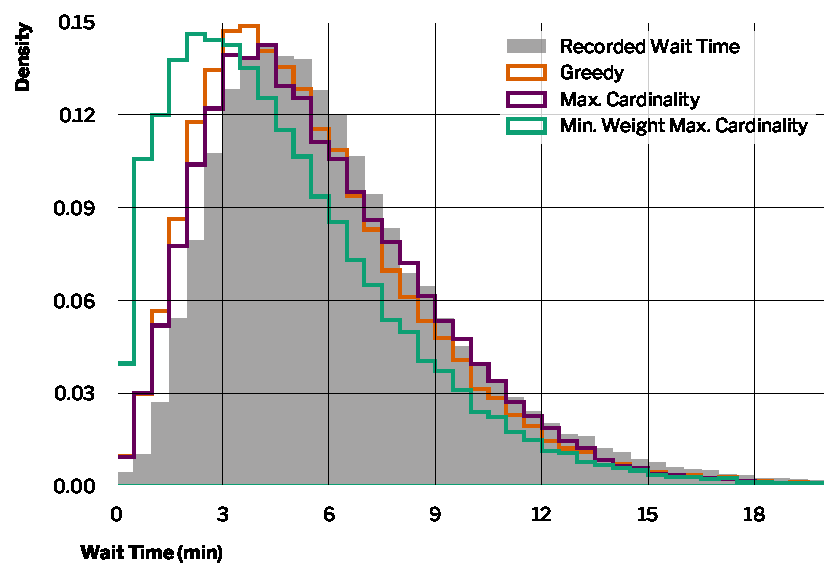
\includegraphics[width=1\textwidth,height=\textheight]{trb_waittime.pdf}
\caption{Recorded distribution of passenger wait times on October 20, 2016, compared
with ones calculated from trip linking using different matching algorithms.
\label{fig:waittime}}
\end{figure}

For both maximum cardinality and greedy matching, we found the optimal \(\delta\)
to be as large as possible (\(\approx20\,\mathrm{min}\), as mentioned in the
methodology). For maximum cardinality, the optimal \(t_\mathrm{batch}\) is as
small as possible (\(1\,\mathrm{min}\), as timestamps after April 2017 are at
best accurate to the minute). Interestingly, the minimum weight maximum
cardinality matching produced a distribution of wait times offset by
\(\sim1.5\,\mathrm{min}\) from the reported distribution regardless of the tuning
parameter values. Between the three matching algorithms, maximum
cardinality produced a distribution closest to the recorded one, and so was
selected to produce our final results in Figure \ref{fig:volfraction}. Since no
wait time data was available for September 13, we use the same parameters as
for October 20.

\hypertarget{testing-and-validating-the-volume-estimation-process}{%
\subsection{Testing and Validating the Volume Estimation Process}\label{testing-and-validating-the-volume-estimation-process}}

\hypertarget{validating-trip-routing}{%
\subsubsection{Validating Trip Routing}\label{validating-trip-routing}}

Trip routing was validated by comparing routed distance with distance in the
ridesourcing trip records.

For October 20, 2016, the fractional difference between recorded and
routed distance is \(-8\% \pm 17\%\). Both these values change by \(\lesssim4\%\)
if only trips greater than the median distance, trips within downtown Toronto,
or trips during peak commuting hours (7:00 - 10:00 a.m. and 4:00 - 7:00 p.m.),
are considered. The discrepancy can partly be explained by the lack of turn
restrictions, and partly by routing not capturing real-world complications like
queuing to turn at intersections, or circling to find an appropriate curbside
location to drop-off a passenger. The standard deviation is also inflated from
\(\sim6\%\) of trips where the fractional difference is greater than \(-33\%\).
Some of these appear to be tours of errands returning to their origin.

To reduce the fractional difference between linked and recorded results, we
aggregated to the Toronto neighbourhood level (\(\sim 2\;\mathrm{km}\) across).
The fractional difference between recorded and routed aggregate VKT within
different neighbourhoods is \(-7 \pm 2\) (\(-6 \pm 4\) for morning
commuting hours and \(-8 \pm 4\) for afternoon commuting).

\hypertarget{validating-trip-linking}{%
\subsubsection{Validating Trip Linking}\label{validating-trip-linking}}

Trip linking was validated by comparing features of the generated results with
reported values from the ridesourcing companies.

\hypertarget{number-of-unique-drivers-per-hour}{%
\paragraph{\texorpdfstring{\emph{Number of Unique Drivers per Hour --}}{Number of Unique Drivers per Hour --}}\label{number-of-unique-drivers-per-hour}}

A subset of ridesourcing companies provided the number of unique drivers per
hour for a set of 39 days from December 2017 - March 2019. An ordinary least
squares regression of the number of active drivers versus the number of
trips gave:
\begin{equation}N_\mathrm{Drivers} = 0.475 N_\mathrm{Trips} + 199.1\label{eq:nvehfit}\end{equation}

\noindent (adjusted \(R^2\) = 0.962; RMS deviation \(= 274.7\)). This is equivalent
to about two trips per driver per hour, though it does not account for drivers
working for multiple ridesourcing companies and therefore slightly
overestimates the number of drivers required to service trips from all
companies in an hour.

\begin{figure}
\centering
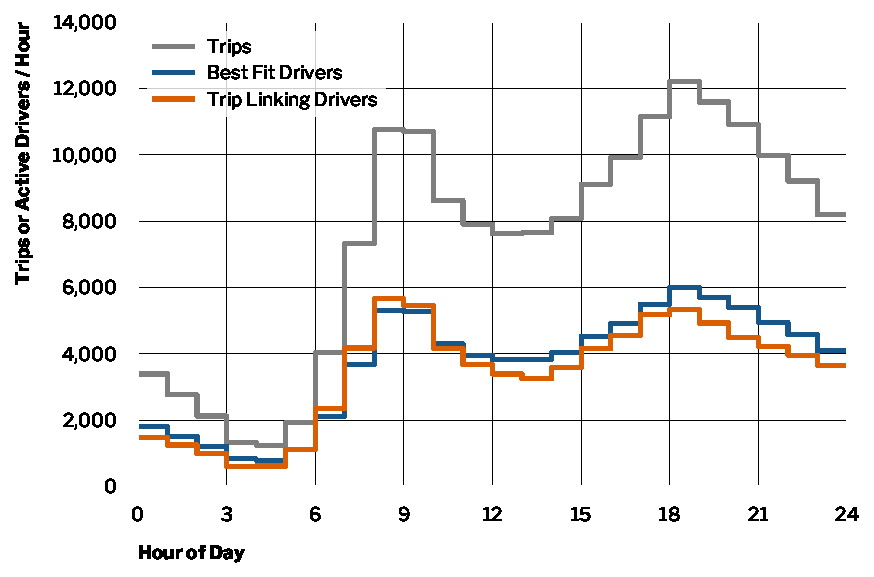
\includegraphics[width=1\textwidth,height=\textheight]{trb_activedrivers.pdf}
\caption{The number of trips per hour on September 13, 2018 and the number of
unique drivers per hour servicing the trips as estimated by a best fit to the
empirical data (Equation \ref{eq:nvehfit}) and trip linking using the maximum
cardinality matching algorithm.
\label{fig:tripsperhour}}
\end{figure}

In Figure \ref{fig:tripsperhour}, we show the number of trips per hour on September
13, 2018, and compare the number of unique drivers predicted by Equation
\ref{eq:nvehfit} and by trip linking. Trip linking reproduces well the two-humped
shape of the best fit curve, but on average predicts \(\sim10\%\) fewer drivers
per hour, which in the evening peak is a deficit of \(\sim500 - 800\) drivers.
The trip linking driver number estimate for October 20, 2016 is also several
hundred fewer drivers than the best fit one, but since there were only half as
many trips on October 20 as there were on September 13, the fractional deficit
is \(\sim25\%\).

\hypertarget{deadheading-as-a-fraction-of-total-activity}{%
\paragraph{\texorpdfstring{\emph{Deadheading as a Fraction of Total Activity --}}{Deadheading as a Fraction of Total Activity --}}\label{deadheading-as-a-fraction-of-total-activity}}

A subset of ridesourcing companies also provided the fraction of their
fleetwide aggregate VKT spent deadheading, reporting that \(55\%\) of total VKT
is for in-service driving, \(35-40\%\) is cruising, and \(5-10\%\) en-route
driving. This means for each kilometer driven in-service, drivers typically
travel an additional \(0.6 - 0.7\) kilometers cruising, and \(0.1 - 0.2\)
kilometers en-route to their next trip.

The ratio of aggregate en-route to in-service VKT from maximum cardinality trip
linking is \(0.15\) for both October 20, 2016 and September 13, 2018, consistent
with the ridesourcing companies' records. However, the records show that
deadheading is dominated by cruising, and while trip linking does not calculate
a cruising VKT, we can estimate it by assuming the ratio of aggregate cruising
to in-service time is roughly the same as the ratio of distances. The
time ratios are sensitive to linking algorithm choice, and for September
13, 2018 range from \(0.16\) for maximum cardinality to only \(0.09\) for greedy
matching. Regardless of algorithm, though, the ratio is always far lower
than reported by the ridesourcing companies. Note that it is unclear whether
they includes drivers making trips unrelated to ridesourcing while keeping
their ridesourcing app open, which would inflate their cruising fraction.

\hypertarget{sec:assessment}{%
\subsection{Assessing the Volume Estimation Process}\label{sec:assessment}}

Given that we did not have to specify anything about the size or behavior of
the ridesourcing driver population, it is remarkable that trip linking is able
to approximate both the passenger wait time distribution (Figure
\ref{fig:waittime}) and number of drivers per hour (Figure \ref{fig:tripsperhour}).
That said, all combinations of linking algorithms and parameters underestimate
the median passenger wait time by at least \(20\,\mathrm{sec}\), and the number
of drivers by at least \(10\%\). Moreover, it grossly underestimates the time
vehicles spend cruising. All these point to trip linking significantly
underestimating deadheading time and VKT. We therefore caution that our volumes
on streets estimates are conservative.

It is possible that some of the assumptions underlying trip linking lead to
unrealistic minimization of deadheading -- most notably, the minimum
weight maximum cardinality algorithm leads to a significant underestimate of
the passenger wait time (Figure \ref{fig:waittime}). One way of more realistically
modelling ridesourcing inefficiencies would be to treat drivers as
agents that stop working after a set time, or after a particularly long trip.
Currently there is no maximum length of time for a work period, and \(10\%\) of
periods from October 10, 2016 are longer than \(4.6\,\mathrm{hrs}\). Another
possibility is that we need to explicitly model cruising behaviour -- perhaps
circling or driving to another neighbourhood during cruising lengthens its
duration. Implementing these features is a promising avenue for future work,
though more empirical data on ridesourcing driver behaviour is required.

One reason we believe agent-based modelling is promising is the work of
\trbcite{calderontrb}, who developed a prototype ridesourcing provision model
using the ridesourcing trip records. Their model is agent-based, and uses
recorded trip \emph{request} times to link drivers and passengers, without requiring
that the driver also arrive at the recorded pick-up time. They also instantiate
drivers randomly throughout the city for deadheading before the first trip, and
use a different method to determine en-route travel times than we do. While our
method is better able to reproduce the recorded passenger wait time distribution,
their aggregate fractional VKT values -- \(39\%\) cruising, \(19\%\) en-route and \(42\%\)
in-service -- are much closer to trip record values, and they are able to
roughly reproduce wait times and drivers per hour using fewer trip record
attributes than we do. A comparative study will be required to understand which
differences between our models is most responsible for producing these
differences.

\hypertarget{sec:results}{%
\section{Results}\label{sec:results}}

This section highlights the key results from our analyses, focussing on
congestion and curbside activity.

Ridesourcing trips have grown rapidly since September 2016, when the service
was first licensed by the City. An average of 176,000 trips were made daily in
March 2019, an increase of over 180\% since September 2016. As of March 2019,
105 million ridesourcing trips have been completed in the City of Toronto.

Ridesourcing trip-making peaks are observed in two distinct time periods:

\begin{itemize}
\tightlist
\item
  \textbf{Friday and Saturday Nights:} the busiest periods are Friday and Saturday
  nights, peaking at an average 13,100 trips per hour at midnight on Sunday
  morning. This time period is typically associated with nightlife activity,
  which is reflected in the dominance of trips in the downtown Entertainment
  District during this time.
\item
  \textbf{Weekday Commuting Periods:} ridesourcing is heavily used in the morning
  and afternoon peak periods, typically associated with the times during which
  the road network experiences the most traffic. This trip market has increased
  over the past two years.
\end{itemize}

\hypertarget{ridesourcing-trips-are-more-commuter-focused-outside-of-downtown}{%
\subsection{Ridesourcing trips are more commuter-focused outside of Downtown}\label{ridesourcing-trips-are-more-commuter-focused-outside-of-downtown}}

\begin{figure}
\centering
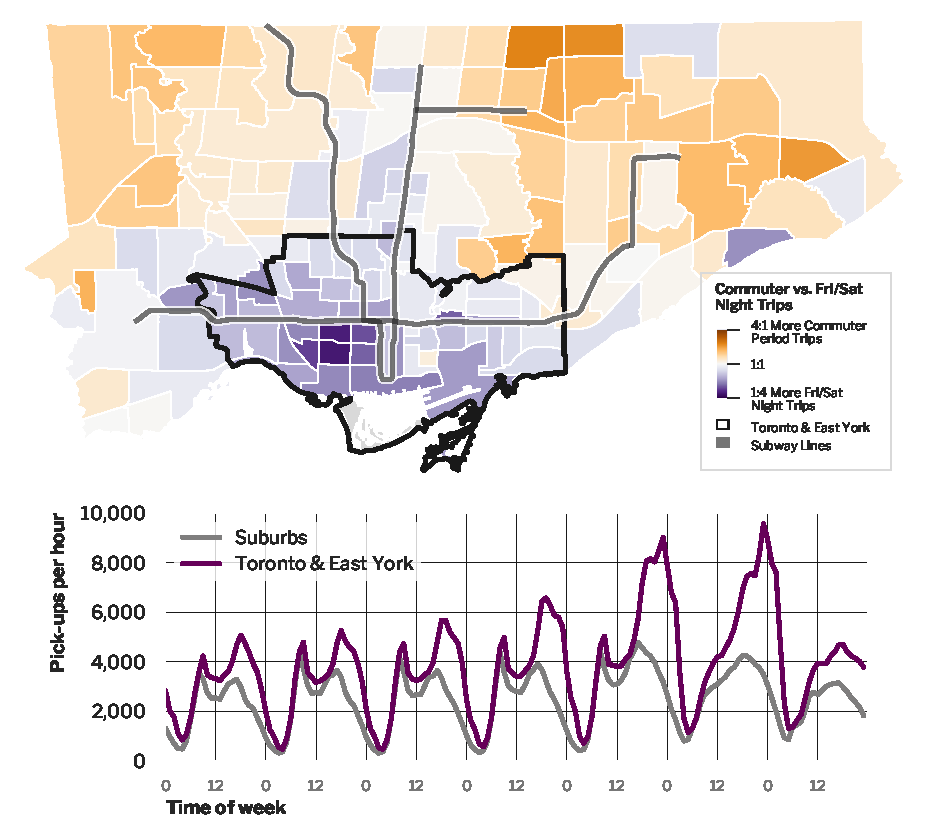
\includegraphics[width=1\textwidth,height=\textheight]{trb_commute_tow.pdf}
\caption{Average ridesourcing pick-ups by neighbourhood and time in September 2018.
Above: a map of the ratio of commuter to Friday/Saturday night trips. The
district of Toronto East York is outlined in black, and the subway system in
gray. Below: number of pick-ups per hour within and outside of Toronto East
York over the course of the week. \label{fig:commtow}}
\end{figure}

Commuter trips are emerging as a major trip market that are being increasingly
captured by ridesourcing. This is illustrated in Figure \ref{fig:commtow},
which shows a landscape with two distinct geographies: downtown neighbourhoods
generally see more than two Friday and Saturday night trips (7 p.m. to 3 a.m.)
for every weekday commuter period (weekdays 7 a.m. to 10 a.m. and 4 p.m. to 7
p.m.) trip while the opposite is true in the suburbs where trips are much more
commuter-focused. Figure \ref{fig:commtow} also compares the average hourly
pick-ups by hour of week for September for the downtown district of Toronto and
East York, and the three suburban districts combined. Trip rates are similar
between the two geographies weekdays from 4 a.m. until 8 a.m., when they peak
in the suburbs. Approximately half of these trips are to the nearest subway
station (10\%) or within their district (40\%), the other half are to other
suburban districts (40\%) or to downtown (10\%). This demonstrates that a portion
of ridesourcing service is helping bring passengers to subway service while
alleviating concerns that they are enabling significant volumes of commuters to
be driven downtown during the peak.

For trips starting downtown, the a.m. peak occurs an hour later at nearly 5,000
trips/hr. This is also an hour later than peak transit ridership according to
the Transportation Tomorrow Survey \cite{wenting2019transitcharacteristics}.
This is when ride-sourcing is least competitive with transit, with travel time
savings of on average 8 min/trip. 73\% of these trips would have been one-seat
rides had they been taken \cite{wenting2019transitcharacteristics}.

The suburban afternoon peak is as high as the morning peak if a little wider.
Downtown the afternoon peak continues into the evening, bolstered by evening
entertainment trips.

\hypertarget{ridesourcing-in-downtown-toronto-make-up-5-8-of-total-traffic}{%
\subsection{Ridesourcing in Downtown Toronto make up 5-8\% of total traffic}\label{ridesourcing-in-downtown-toronto-make-up-5-8-of-total-traffic}}

Figure \ref{fig:volfraction} shows our conservative estimate of ridesourcing
volumes which does not include cruising estimates. The largest volumes of
ridesourcing vehicles are concentrated downtown where they account for
between 5 and 8\% of overall daily traffic in downtown neighbourhoods. The
busiest neighbourhood is Waterfront Communities-The Island, which includes major
transportation nodes such as Union Station and Billy Bishop Airport.

On this day, ridesourcing accounted for approximately 1,230,000 VKT. This is
estimated to be 1.9\% of the total 67,200,000 VKT traveled in Toronto on average.
The proportion of traffic in a.m. and p.m. peak commuting periods is slightly
lower than the overall daily totals, reflecting the higher relative ridesourcing
volumes that occur during evening hours.

\begin{figure}
\centering
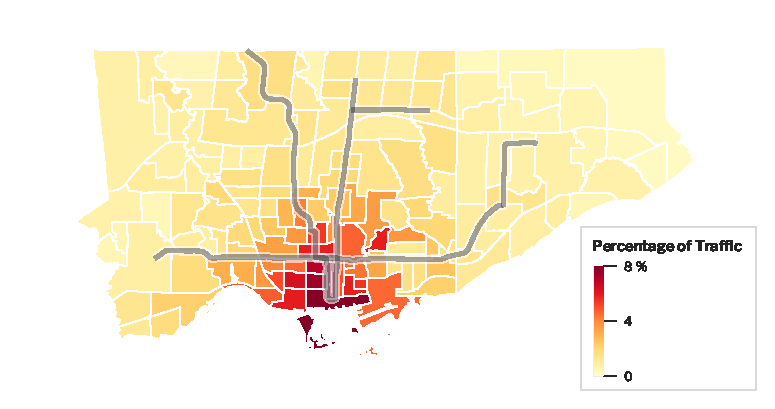
\includegraphics[width=1\textwidth,height=\textheight]{trb_volfraction.pdf}
\caption{Percentage of total City VKT due to ridesourcing activity for September 13,
2018. Only in-service and en-route VKT are included (see Methods)
\label{fig:volfraction}}
\end{figure}

\hypertarget{downtown-travel-times-have-been-stable-over-18-months-while-ridesourcing-trips-increased-by-96}\label{downtown-travel-times-have-been-stable-over-18-months-while-ridesourcing-trips-increased-by-96}}

Figure \ref{fig:bt_traveltime} shows the percent change in average travel time
based on Bluetooth sensor readings on most major streets in the downtown core,
the area of the City where ridesourcing trip concentrations are highest. This
data shows marginal changes in travel times over the 18 months from October
2017 to March 2019 in the downtown core. Travel times on major streets have
increased by 4\% in the morning peak hour (7 to 10 a.m.), and decreased by 1\% in
both the afternoon peak period (4 to 7 p.m.) and Friday and Saturday nights (10
p.m. to 1 a.m.). Over this same span, ridesourcing trips increased 96\%
city-wide, from 83,800 to 164,000 daily trips.

\begin{figure}
\centering
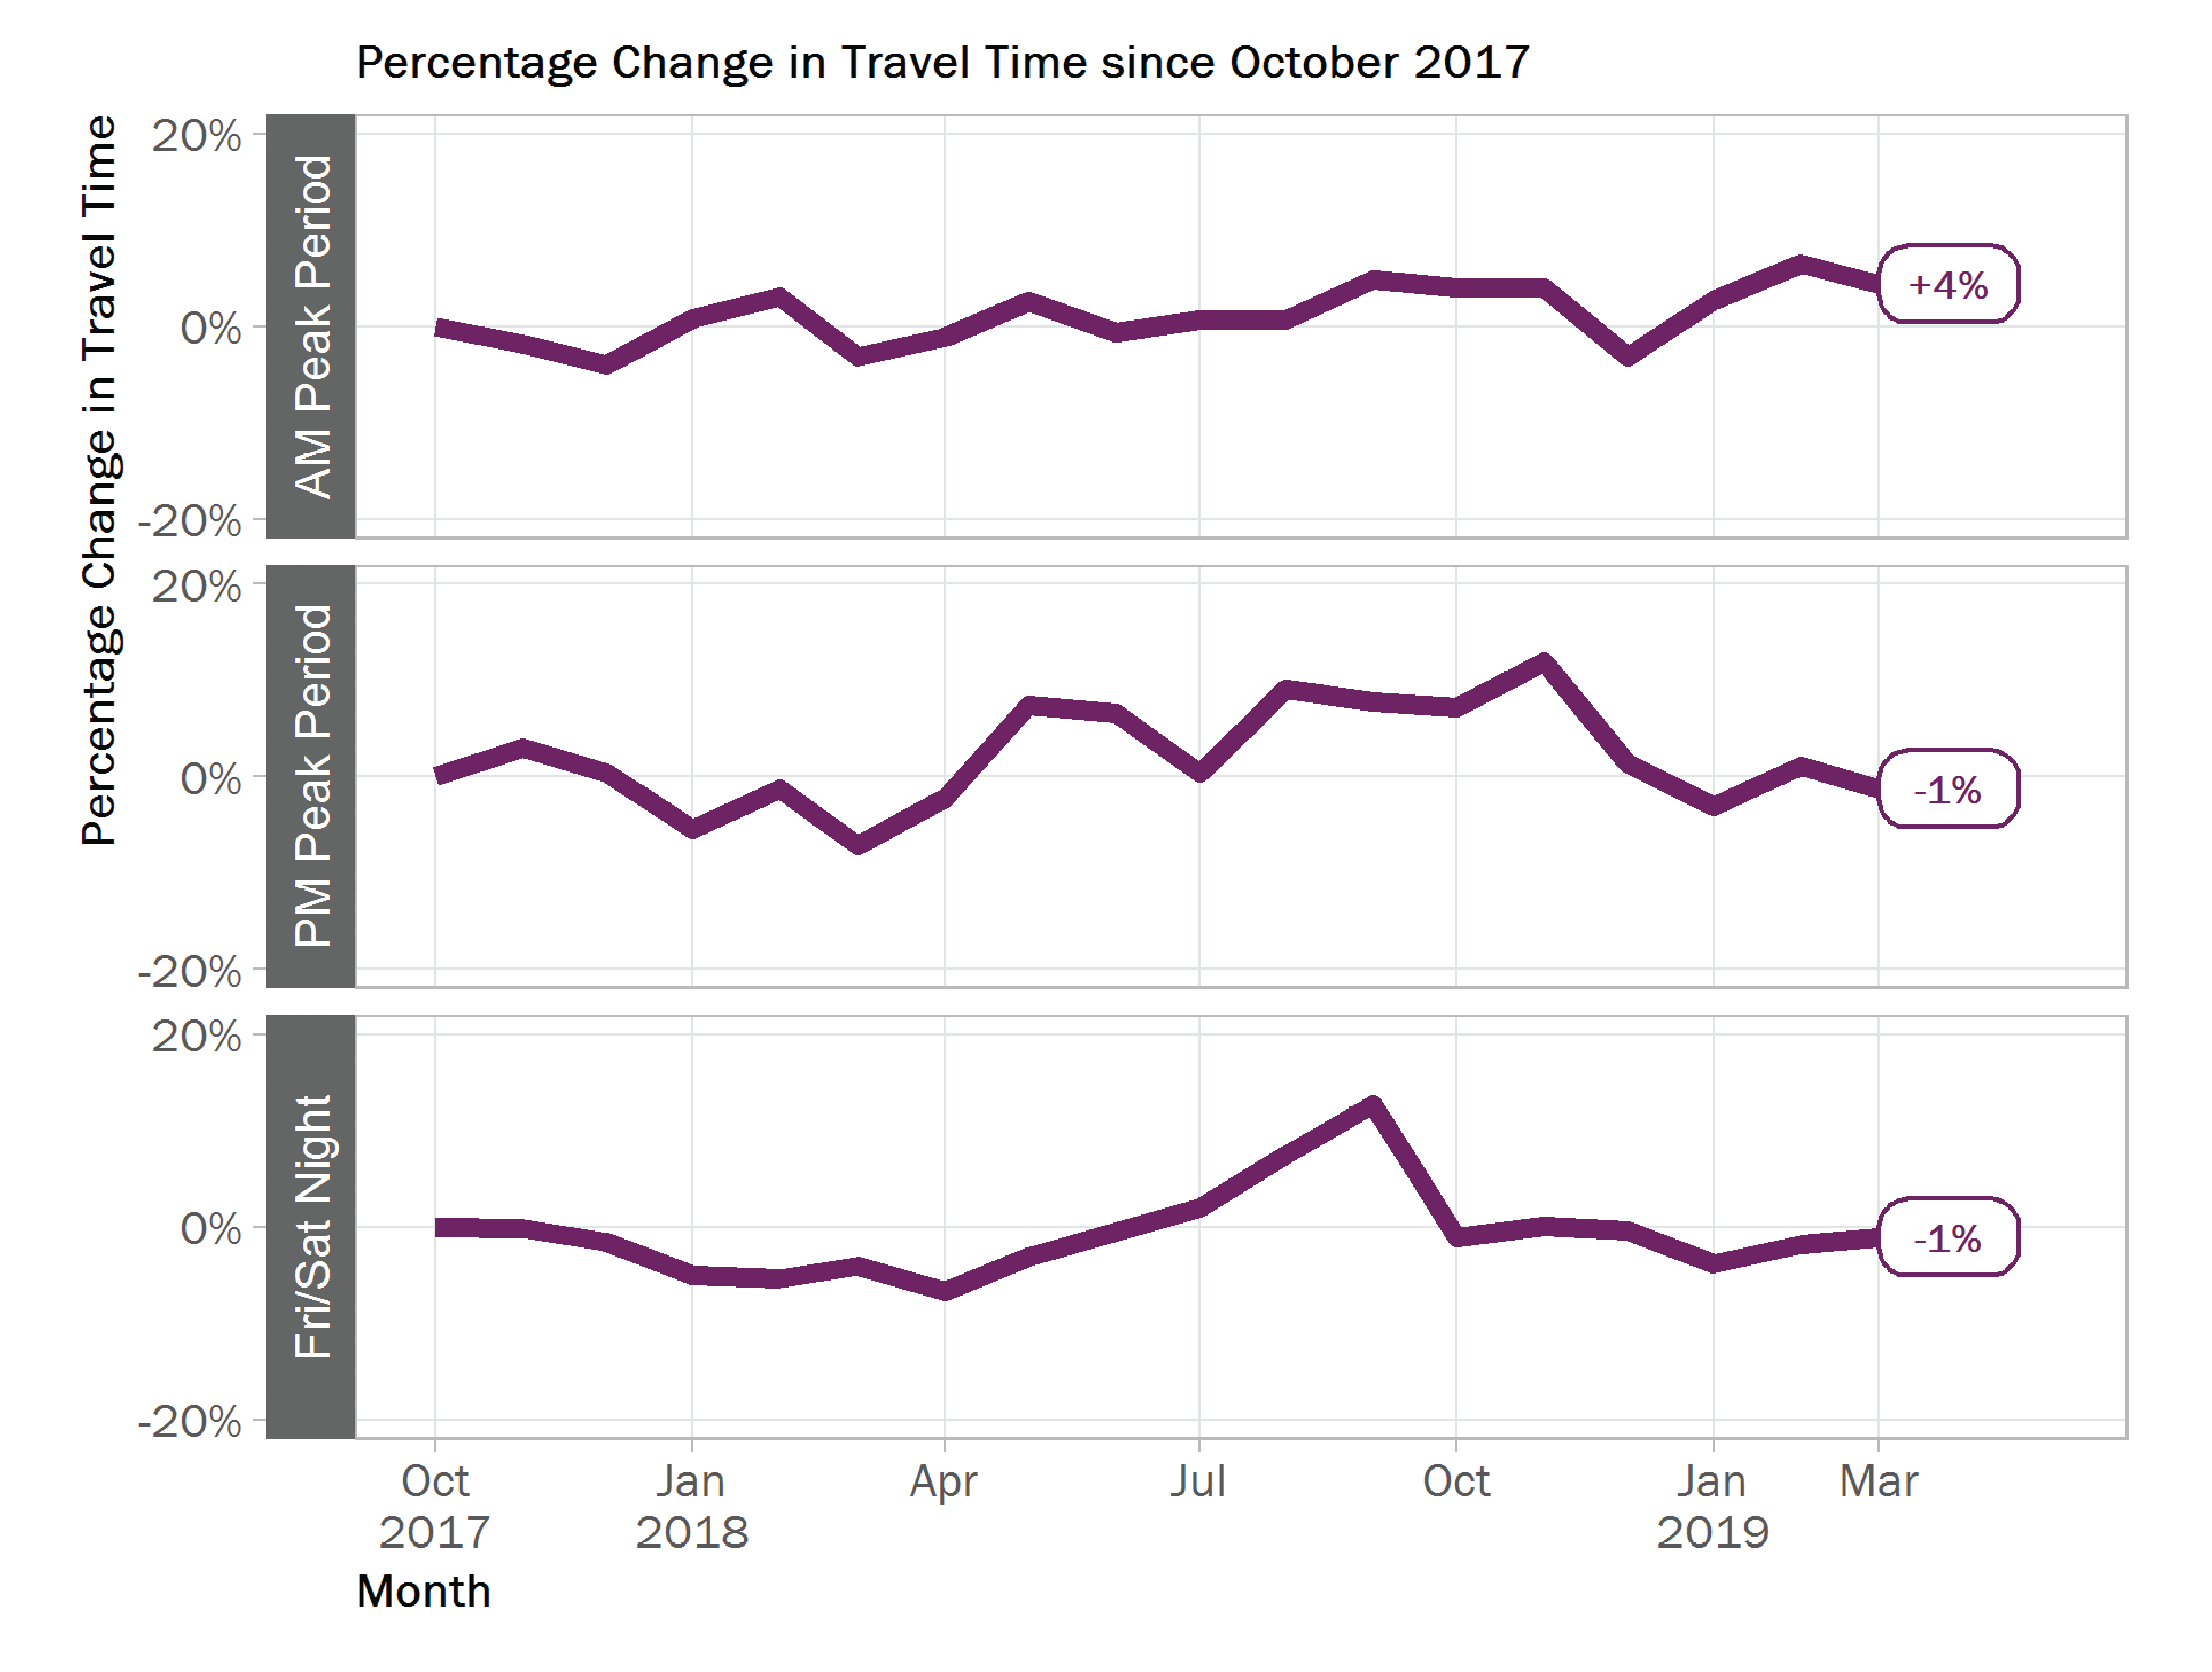
\includegraphics[width=1\textwidth,height=\textheight]{trb_bt_traveltime.pdf}
\caption{Monthly average travel time in Toronto's downtown core for the a.m. and p.m.
commute periods, and for Friday/Saturday night. Times are normalized to their
October 2017 averages to highlight fractional changes.
\label{fig:bt_traveltime}}
\end{figure}

Given that changes in travel times have been negligible in the neighbourhoods
where ridesourcing makes up the largest proportions of overall traffic, there
is insufficient evidence at this time to make any definitive linkages between
ridesourcing volumes and changes in travel time.

\hypertarget{pick-up-and-drop-off-data-highlight-conflicts-with-no-stopping-zones-and-bike-lanes}{%
\subsection{Pick-up and drop-off data highlight conflicts with no-stopping zones and bike lanes}\label{pick-up-and-drop-off-data-highlight-conflicts-with-no-stopping-zones-and-bike-lanes}}

\begin{figure}
\centering
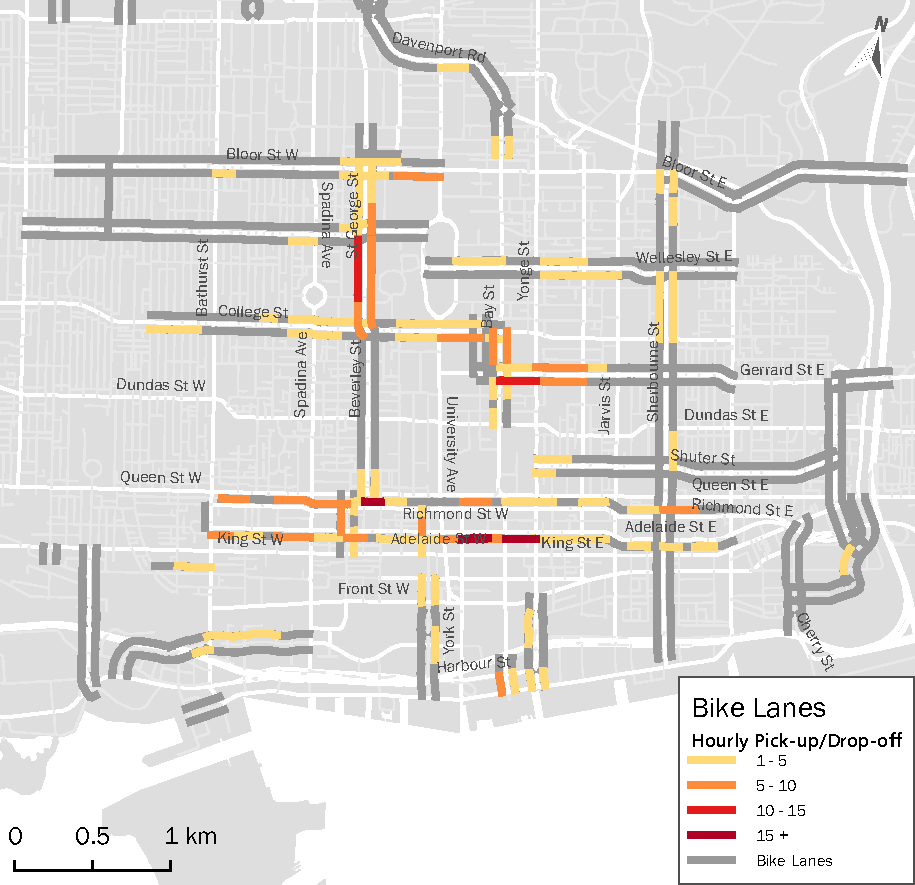
\includegraphics[width=1\textwidth,height=\textheight]{trb_bikeconflict.pdf}
\caption{Hourly average number of ridesourcing pick-ups and drop-offs adjacent to bike
lanes and separated bike facilities between 7 a.m. and 7 p.m. Data is averaged
from Monday, September 10 to Thursday, September 13, 2018.
\label{fig:bikeconflict}}
\end{figure}

A particular safety concern with ridesourcing pick-up and drop-off activity is
potential conflicts with cyclists, especially when it occurs in close proximity
to cycling infrastructure. A detailed look at pick-up/drop-off data has shown hotspots during the morning
commute period where pick-up and drop-off activity is occurring in no-stopping
zones. The largest hotspots are in the Financial District. Figure
\ref{fig:bikeconflict} shows a similar analysis of pick-ups and drop-offs
adjacent to bike lanes and separated bike facilities between 7 a.m. and 7 p.m.
during a typical weekday in September 2018. There is a significant volume of
pick-up and drop-off activity near high-use bike facilities. This highlights
locations that could benefit from additional separation between bike lanes and
vehicular traffic. Despite the greater accuracy of the positions, it is
impossible to conclude from this data whether the ridesourcing vehicle was
within or adjacent to a bike lane while picking up or dropping off passengers.
Nevertheless, these hotspots indicate where they may be a high risk of
conflicts.

\hypertarget{sec:discussion}{%
\section{Discussion}\label{sec:discussion}}

This section presents the results and outcomes of this study in context with
other regulatory analyses.

\hypertarget{sec:congestion}{%
\subsection{Congestion}\label{sec:congestion}}

A comparison of ridesourcing VMT as a proportion of total VMT with other cities
that have performed similar studies shows that Toronto is at an earlier stage
of maturity. The TNCs Today report by the SFCTA estimated VMT from ridesourcing
vehicles to be at 6.5\% of city-wide weekday VMT \cite{tncstoday} in 2016. A
2019 report by the NYC Taxi and Limousine Commission and the NYC Department of
Transportation estimates 30\% of VMT in Manhattan can be attributed to
ridesourcing vehicles \cite{nyctlc2019report}. The same report recommends
continuing the freeze on issuing new licenses to ridesourcing drivers and
requiring ridesourcing companies to reduce cruising (any time spend with the
ridesourcing app on but without passengers) as a percentage of driving time to
31\% in Manhattan.

\hypertarget{sec:curbside-management}{%
\subsection{Curbside Management}\label{sec:curbside-management}}

A number of cities have implement dedicated passenger loading/unloading zones
to respond to growing demand for curb space, to reduce conflicts with competing
uses for curb access, and as part of their Vision Zero programs. These include
\trbcite{westhollywoodcurb} and Washington, D.C. \cite{ddotcurb}. The City of
Toronto will use pick-up/drop-off (PUDO) data to inform the design of bike
infrastructure and inform prioritization of infrastructure upgrades. Further
study would be required to determine how designated passenger loading zones
could be implemented and how providing digitized curb regulation data could
better manage curb utilization. Additional monitoring and analysis is needed to
better understand the extent of conflicts between cyclists and pick-up and
drop-off activity and to determine if this activity correlates with improved
cycling comfort and reduced rates of cyclist conflicts.

\hypertarget{sec:conclusion}{%
\section{Conclusion}\label{sec:conclusion}}

This study has looked at what is most-likely the first wave of disruptions from
new mobility businesses in Toronto. Trip growth is not anticipated to slow in
the upcoming years and these services will likely create traffic and
operational challenges throughout the City in the future. However, the rapid
growth in trips demonstrates ridesourcing services have been immensely popular
with Toronto residents. They now play an important role in many residents'
daily travel patterns including an increasing role in daily commuter travel.

An executive summary of the Transportation Impacts of Vehicle-for-Hire report was
attached to the Staff Report prepared by Municipal Licensing \& Standards and
presented to the General Governance \& Licensing committee on June 24, 2019.
Councillors requested we report on the number of ride-sourcing vehicles
operating and to elaborate on our findings regarding congestion. The report and
these additional analyses were discussed at City Council on July 18th.
Council approved staff recommendations, with amendments. The following relevant
regulations were approved:

\begin{itemize}
\tightlist
\item
  Request that taxi/ridesourcing be a field on the standardized collision
  reporting form. Require that all vehicle for hire brokerages and companies
  report collision incidents.
\item
  Create an accessibility fund to encourage the purchases of accessible
  vehicles.
\item
  Require that all vehicle for hire drivers receive driver training.
\item
  Require additional data to be provide by ridesourcing companies: aggregate
  vehicle volumes in geographic areas, pick-up and drop-off data at a
  \(10\,\mathrm{m}\) resolution, aggregate number of vehicles having completed
  trips by hour.
\item
  Require that taxi brokerages provide similar trip record data as ridesourcing
  companies
\end{itemize}

Council further required Transportation Services to report in 2020 on whether
there has been an impact on congestion from vehicles for hire, what mitigating
measures can be taken, and determine the appropriate number of vehicles for
hire. Council also required a report on the safety of ridesourcing operations
and the feasibility of requiring vehicle for hire applications to route them
such that they do not stop to pick-up or drop-off passengers in ``no stopping''
zones.

The goal of the Transportation Impact Study was to build a deeper understanding
of these new services and to pave the way for future work and studies to keep
in front of these rapidly changing trends. This will allow the City to define
policy to support the benefits of ridesourcing services while minimizing
adverse impacts to traffic, to the environment and to the equity of mobility
services.

Having performed this comprehensive study, we claim that transportation
agencies need three important datasets to be derived from ridesourcing
activity, each which its own utility for regulation:

\begin{itemize}
\tightlist
\item
  \textbf{Trip OD records:} for transportation planning;
\item
  \textbf{Ridesourcing vehicle volumes:} for congestion management; and
\item
  \textbf{Pick-up/drop-off activity:} for curbside management and vision zero
  planning.
\end{itemize}

For the purposes of this study we were provided trip records and PUDO data, and
we presented a novel process to derive vehicle volumes from trip records which
other agencies could use.

\hypertarget{sec:acknowledgments}{%
\section{Acknowledgments}\label{sec:acknowledgments}}

The authors confirm contribution to the paper as follows: study conception and
design: Raphael Dumas, Jesse Coleman, Charles Zhu; data collection: Raphael
Dumas, Rick Liu; analysis and interpretation of results: contributions from all
authors; draft manuscript preparation: Raphael Dumas, Charles Zhu. All authors
reviewed the results and approved the final version of the manuscript.

The authors would like to thank Cathy Nangini and Chelsea Rosic, of the Big
Data Innovation Team, for their contributions to the Transportation Impacts
Study which were not included in this paper. They would also like to thank the
research team at the University of Toronto Transportation Research Institute
led by Professors Miller, Habib, and Shalaby for their research, insight, and
contributions to this study.

\begin{thebibliography}{33}
\raggedright
\providecommand{\natexlab}[1]{#1}

\bibitem[{Schneider(2019)}]{schneider2019dashboard}
Schneider, T.~W., \emph{Taxi and Ridehailing Usage in New York City}.
  \url{https://toddwschneider.com/dashboards/nyc-taxi-ridehailing-uber-lyft-data}.
  Accessed July 17, 2019.

\bibitem[{{City of Chicago}(2019)}]{chicago2019transportation}
{City of Chicago}, \emph{Transportation Network Providers - Trips}.
  \url{https://data.cityofchicago.org/Transportation/Transportation-Network-Providers-Trips/m6dm-c72p}.
  Accessed July 17, 2019.

\bibitem[{Cooper et~al.(2018)Cooper, Castiglione, Mislove, and
  Wilson}]{cooper2018profiling}
Cooper, D., J.~Castiglione, A.~Mislove, and C.~Wilson, Profiling Transport
  Network Company Activity using Big Data. \emph{Transportation Research
  Record}, Vol. 2672, No.~42, 2018, pp. 192--202.

\bibitem[{Henao and Marshall(2018)}]{henao2018impact}
Henao, A. and W.~E. Marshall, The impact of ride-hailing on vehicle miles
  traveled. \emph{Transportation}, 2018, pp. 1--22.

\bibitem[{{Ride Austin}(2017)}]{rideaustin2017data}
{Ride Austin}, \emph{Ride-Austin-june6-april13}.
  \url{https://data.world/ride-austin/ride-austin-june-6-april-13}. Accessed
  April 12, 2019.

\bibitem[{{New York City Taxi and Limousine Commission} and {New York City
  Department of Transportation}(2019)}]{nyctlc2019report}
{New York City Taxi and Limousine Commission} and {New York City Department of
  Transportation}, \emph{Improving Efficiency and Managing Growth in New York's
  For-Hire Vehicle Sector}.
  \url{https://www1.nyc.gov/assets/tlc/downloads/pdf/fhv_congestion_study_report.pdf},
  New York City Taxi and Limousine Commission, 2019.

\bibitem[{{City of Toronto}(2019)}]{vfhbylaw}
{City of Toronto}, \emph{TORONTO MUNICIPAL CODE CHAPTER 546, LICENSING OF
  VEHICLES-FOR-HIRE}.
  \url{https://www.toronto.ca/legdocs/municode/toronto-code-546.pdf}, 2019,
  accessed July 30, 2019.

\bibitem[{{Big Data Innovation Team} and {University of Toronto Transportation
  Research Institute}(2019)}]{bdittoreport}
{Big Data Innovation Team} and {University of Toronto Transportation Research
  Institute}, \emph{The Transportation Impacts of Vehicle-for-Hire in the City
  of Toronto}.
  \url{https://www.toronto.ca/wp-content/uploads/2019/06/96c7-Report_v1.0_2019-06-21.pdf},
  City of Toronto, 2019.

\bibitem[{Loa et~al.(2019)Loa, Hawkins, and Habib}]{loatrb}
Loa, P., J.~Hawkins, and K.~N. Habib, Use of ``SP-off-RP'' Experiment to
  Understand the Impacts and Utilization of Ride-Hailing Services and the
  Determinants of Mode Choice: The case of the City of Toronto. \emph{Submitted
  to Transportation Research Record}, 2019.

\bibitem[{Li et~al.(2019{\natexlab{a}})Li, Shalaby, and
  Habib}]{wenting2019transitcharacteristics}
Li, W., A.~Shalaby, and K.~N. Habib, Comparative Analysis of the Travel
  Characteristics between Ride-Hailing and Public Transit in Toronto.
  \emph{Submitted to Transportation Research Record}, 2019{\natexlab{a}}.

\bibitem[{Li et~al.(2019{\natexlab{b}})Li, Shalaby, and
  Habib}]{wenting2019transitcompetition}
Li, W., A.~Shalaby, and K.~N. Habib, Exploring the Ridership Impacts of
  Ride-hailing on Multimodal Public Transit in Toronto. \emph{Submitted to
  Transportation Research Record}, 2019{\natexlab{b}}.

\bibitem[{Calder\'{o}n and Miller(2019)}]{calderontrb}
Calder\'{o}n, F. and E.~J. Miller, A Prototype Model of Ridehailing Service
  Provision. \emph{Submitted to Transportation Research Record}, 2019.

\bibitem[{Erhardt et~al.(2019)Erhardt, Roy, Cooper, Sana, Chen, and
  Castiglione}]{Erhardteaau2670}
Erhardt, G.~D., S.~Roy, D.~Cooper, B.~Sana, M.~Chen, and J.~Castiglione, Do
  transportation network companies decrease or increase congestion?
  \emph{Science Advances}, Vol.~5, No.~5, 2019.

\bibitem[{{New York City Office of the Mayor}(2016)}]{nyc2016report}
{New York City Office of the Mayor}, \emph{For-Hire Vehicle Transportation
  Study}.
  \url{https://www1.nyc.gov/assets/operations/downloads/pdf/For-Hire-Vehicle-Transportation-Study.pdf},
  New York City Office of the Mayor, 2016.

\bibitem[{cen(2019)}]{centrelinexsection}
\emph{Intersection File - City of Toronto}.
  \url{https://open.toronto.ca/dataset/intersection-file-city-of-toronto/},
  2019, accessed July 30, 2019.

\bibitem[{{SharedStreets}(2019)}]{sharedstreetsactivity}
{SharedStreets}, \emph{Taxi and TNC Activity}.
  \url{https://sharedstreets.io/taxi-tnc-activity/}, 2019, accessed July 30,
  2019.

\bibitem[{Reddy et~al.(2019)Reddy, Ganji, Abiola, and
  Hatzopoulou}]{volumemodel}
Reddy, B. R.~C., A.~Ganji, S.~Abiola, and M.~Hatzopoulou, \emph{Analyzing the
  Effects of Transit-Only Corridors on Traffic and Emissions in the Affected
  Neighbourhoods: A Before-After Intervention Analysis}. Presented at 98th
  Annual Meeting of the Transportation Research Board, Washington, D.C., 2019.

\bibitem[{{The PostgreSQL Global Development Group}(2019)}]{postgres}
{The PostgreSQL Global Development Group}, \emph{{PostgreSQL}}.
  \url{https://www.postgresql.org}. Accessed July 17, 2019.

\bibitem[{{PostGIS Project}(2019)}]{postgis}
{PostGIS Project}, \emph{{PostGIS}}. \url{https://postgis.net}. Accessed July
  16, 2019.

\bibitem[{Eros(2019)}]{sharedstreetshowtomatch}
Eros, E., \emph{How the SharedStreets Referencing System Works}.
  \url{https://sharedstreets.io/how-the-sharedstreets-referencing-system-works/}.
  Accessed July 30, 2019.

\bibitem[{{pgRouting Project}(2019)}]{pgrouting}
{pgRouting Project}, \emph{{pgRouting}}. \url{https://pgrouting.org}. Accessed
  July 16, 2019.

\bibitem[{Anderson(2014)}]{anderson2014not}
Anderson, D.~N., ``Not just a taxi''? For-profit ridesharing, driver
  strategies, and VMT. \emph{Transportation}, Vol.~41, No.~5, 2014, pp.
  1099--1117.

\bibitem[{Gurley(2014)}]{gurley2014dynamic}
Gurley, B., \emph{A Deeper Look at Uber's Dynamic Pricing Model}.
  \url{http://abovethecrowd.com/2014/03/11/a-deeper-look-at-ubers-dynamic-pricing-model},
  Above the Crowd. Accessed July 19, 2019.

\bibitem[{{Stanford University School of Engineering}(2018)}]{ubervideo}
{Stanford University School of Engineering}, \emph{Dawn Woodward: How Uber
  matches riders and drivers to reduce waiting time}.
  \url{https://www.youtube.com/watch?v=jZk04aqvzBU}. Accessed July 27, 2019.

\bibitem[{Vazifeh et~al.(2018)Vazifeh, Santi, Resta, Strogatz, and
  Ratti}]{vazifeh2018addressing}
Vazifeh, M.~M., P.~Santi, G.~Resta, S.~Strogatz, and C.~Ratti, Addressing the
  minimum fleet problem in on-demand urban mobility. \emph{Nature}, Vol. 557,
  No. 7706, 2018, p. 534.

\bibitem[{Hanna et~al.(2016)Hanna, Albert, Chen, and Stone}]{hanna2016minimum}
Hanna, J.~P., M.~Albert, D.~Chen, and P.~Stone, Minimum cost matching for
  autonomous carsharing. \emph{IFAC-PapersOnLine}, Vol.~49, No.~15, 2016, pp.
  254--259.

\bibitem[{Boesch and Gimpel(1977)}]{boesch1977covering}
Boesch, F.~T. and J.~F. Gimpel, Covering points of a digraph with
  point-disjoint paths and its application to code optimization. \emph{Journal
  of the ACM (JACM)}, Vol.~24, No.~2, 1977, pp. 192--198.

\bibitem[{{Swart, Pieter and Schult, Dan and Hagberg, Aric}(2019)}]{networkx}
{Swart, Pieter and Schult, Dan and Hagberg, Aric}, \emph{{NetworkX}}.
  \url{https://github.com/networkx/networkx}. Accessed July 27, 2019.

\bibitem[{{Google Operations Research}(2019)}]{ortools}
{Google Operations Research}, \emph{{Google OR-Tools}}.
  \url{https://developers.google.com/optimization}. Accessed July 27, 2019.

\bibitem[{Lin(1991)}]{lin1991divergence}
Lin, J., Divergence measures based on the Shannon entropy. \emph{IEEE
  Transactions on Information theory}, Vol.~37, No.~1, 1991, pp. 145--151.

\bibitem[{{San Francisco County Transportation Authority}(2017)}]{tncstoday}
{San Francisco County Transportation Authority}, \emph{TNCs Today: A Profile of
  San Francisco Transportation Network Company Activity}.
  \url{https://www.sfcta.org/sites/default/files/2019-02/TNCs_Today_112917_0.pdf}.
  Accessed July 29, 2019.

\bibitem[{{City of West Hollywood}(2018)}]{westhollywoodcurb}
{City of West Hollywood}, \emph{THE DROP}.
  \url{https://www.weho.org/city-government/city-departments/facilities-and-recreation-services/parking-services/the-drop}.
  Accessed July 29, 2019.

\bibitem[{{District Department of Transportation}(2018)}]{ddotcurb}
{District Department of Transportation}, \emph{Mayor Bowser and DDOT Announce
  Pick-Up/Drop-Off Zone Pilot Program Expansion}.
  \url{https://ddot.dc.gov/release/mayor-bowser-and-ddot-announce-pick-updrop-zone-pilot-program-expansion}.
  Accessed July 29, 2019.

\end{thebibliography}

\end{document}
